\documentclass[12pt]{article}
\usepackage{geometry}
\geometry{
	letterpaper,
	left=20mm,
	right=20mm,
	top=25mm,
	bottom=30mm,
}
\usepackage{graphicx}
\usepackage{tikz}
\usepackage{tikzscale}
\usepackage{pgfplots}
\usepackage{amsmath,amssymb}
\usepackage{enumitem}
\usepackage{algorithm}
\usepackage{algorithmicx}
\usepackage{algpseudocode}
\usepackage{subcaption}
\usepackage{mathtools}
\usepackage{amsthm}
\usepackage{nccmath} %for fleqn
\makeatletter
\def\verbatim@font{\linespread{1}\normalfont\ttfamily}
\makeatother
\usepackage[breaklinks]{hyperref} 
\hypersetup{
	colorlinks   = true,
	citecolor    = blue
}
\hypersetup{linkcolor=blue}
\usepackage[T1]{fontenc}
\DeclarePairedDelimiter{\ceil}{\lceil}{\rceil}
\mathchardef\mhyphen="2D
\newcommand\makeset{\mathop{make\mhyphen set}}
\newcommand\findset{\mathop{find\mhyphen set}}
\newcommand*{\Comb}[2]{{}^{#1}C_{#2}}
\usepackage{mdframed}
\usepackage{fancyhdr} 
\fancyhf{}
\chead{\courseName}
\lhead{\thepage}  
\rhead{\homeworkName}
\renewcommand{\headrulewidth}{1pt}
\renewcommand{\footrulewidth}{0pt} 
\fancypagestyle{first}{% 
	\fancyhf{} % clear all header and footer fields 
	\chead{
		\small
		} % except the center 
	\renewcommand{\headrulewidth}{0pt} 
	\renewcommand{\footrulewidth}{0pt}
} 
\fancypagestyle{second}{% 
	\fancyhf{} % clear all header and footer fields 
	\chead{} % except the center 
	\renewcommand{\headrulewidth}{0pt} 
	\renewcommand{\footrulewidth}{0pt}
}
\pagestyle{fancy} 
	
\usepackage{xepersian}
\settextfont[
Scale=1.2,
Extension=.ttf, 
Path=../../common/fonts/,
BoldFont=*-BOLD
]{B-NAZANIN}
\setlatintextfont[Scale=1.1]{Times New Roman}
%\setdigitfont[Scale=1.4]{Times New Roman}
\setlength\parindent{0pt}

\newcommand{\courseName}{ارزیابی کارایی سیستم های کامپیوتری}
\newcommand{\courseSemester}{پاییز ۱۴۰۲}
\newcommand{\homeworkName}{تمرین اول}
\newcommand{\homeworkDue}{موعد: }

\renewcommand{\baselinestretch}{1.5} 
\pgfplotsset{compat=1.18}
\begin{document}
    
	\graphicspath{{../../common/cover/},{img/}}
	\pagenumbering{gobble} 
	\thispagestyle{first}
%\newgeometry{top=2cm}
%\newcommand*{\SSS}{\includegraphics[scale=0.2]{ut}}%
%\newcommand*{\TTT}{\includegraphics[scale=0.2]{fanni}}%
\begin{mdframed}
\begin{minipage}[t]{0.2\textwidth}
	\centering
	
\includegraphics[width=0.6\textwidth]{sharif} \\
%	\vspace{0.2cm}
	\homeworkName
\end{minipage}%
\begin{minipage}[b]{0.59\textwidth}
	\centering
	\courseName \\
	\courseSemester
\end{minipage}%
\begin{minipage}[t]{0.2\textwidth}
	\centering
	
\includegraphics[width=0.6\textwidth]{sharif} \\
	\homeworkDue
\end{minipage}%
\end{mdframed}
%\restoregeometry

	\pagenumbering{arabic}  
	در تمرین اول، هر دانشجو باید سوال‌هایی از کتاب مرجع را که به ایشان انتصاب داده‌شده است، انجام دهد. فایل اکسل سوالات انتصاب داده‌شده به دانشجویان در ایلرن قرار دارد.

\textbf{در ارسال تمرین موارد زیر رعایت شود:}

\begin{itemize}
	\item[-]
	 بیان مسئله و پاسخ سوال به طور دقیق و کامل به زبان فارسی نوشته شود.

	\item[-]	
	 نوشته شما باید نشان‌دهد مسئله و جواب را فهمیده‌اید.
	
	\item[-]	
	اگر بتوانید توضیحات اضافی به پاسخ‌تان بیفزایید تا آن را قابل‌ درک‌تر کنید، نمره اضافی دریافت خواهید کرد.
\end{itemize}

\textbf{نکاتی که باید توجه داشته باشید:}

\begin{itemize}
	\item[الف)]
	مهلت ارسال در سربرگ تمرین همچنین در ایلرن درج شده‌است.
	\item[ب)]
	کلیه تمرینات (غیر از تمرینات سرکلاسی) از طریق ایلرن دریافت می‌شوند و دیگر شیوه‌های ارسال تمرین پذیرفته نیست.
	\item[ج)]
	قالب تمرینات به‌صورت \lr{\LaTeX} و تنها در \lr{Template} تمرینات مورد پذیرش است. (\lr{Template} در ایلرن در دسترس است.)
	\item[د)]	
	فایل تمرین ارسالی باید شامل فایل‌های مورد نیاز به جهت اجرای فایل \lr{\LaTeX} به همراه \lr{PDF} باشد. نام فايل را به‌صورت زير انتخاب كنيد:

\begin{latin} \begin{center}
		\texttt{HW1\_Student\#\_Name}
	\end{center}
\end{latin}

	\item[ه)]
	ارسال با تأخیر تمرین، تنها تا سه‌روز پس از مهلت تمرین امکان‌پذیر بوده و به ازای هر روز 5 درصد کسر نمره خواهد داشت. پس از گذشت این مهلت، امکان ارسال تمرین میسر نیست.
\end{itemize}

	\newpage


	\textbf{مسئله اول}
	\newline
	\textit{یک سیستم صف از دو سرور مشابه که به صورت موازی خدمت رسانی انجام می‌دهند تشکیل شده است. در حالت پایداری تعداد مشتری‌ها درون سیستم میان صفر تا چهار نفر تغییر می‌کند. احتمال حضور \lr{n} مشتری در سیستم به صورت زیر است.}
	\begin{center}
	    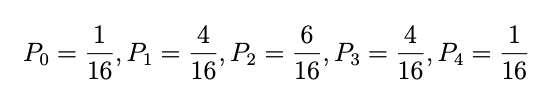
\includegraphics[width=0.6\textwidth]{Content/figure-1.png}
	\end{center}
	\begin{itemize}
	\item[-]
امید ریاضی تعداد مشتریان درون سیستم را مشخص کنید.
	\item[-]	
	 امید ریاضی تعداد مشتریان درون صف را محاسبه کنید (افرادی که سرویس نمی‌گیرند).
	\item[-]	
میانگین تعداد افرادی که درحال سرویس هستند را بدست آورید.
	\item[-]	
میانگین زمان انتظار در سیستم و میانگین زمان انتظار در صف را محاسبه کنید. (با فرض اینکه نرخ ورود مشتری ۲ نفر در ساعت باشد)
	\item[-]	
با فرض اینکه هر دو سرور دارای میانگین زمان سرویس مشابهی هستند، با استفاده از نتایج بخش قبل زمان سرویس را محاسبه کنید.
    \end{itemize}
    \bigskip

    \textbf{مسئله دوم}
	\newline
	\textit{مشتری‌های یک سیستم طبق یک فرآیند پوآسون وارد می‌شوند. میانگین نرخ ورود دو مشتری در ساعت است. فرض کنید
که سیستم دچار اشکال می‌شود و یک ساعت برای تعمیر آن طول می‌کشد. احتمال اینکه در این بازه تعداد مشتری‌های جدید که مراجعه می‌کنند برابر با ۱) صفر ۲) دو ۳) پنج نفر یا بیشتر باشد را محاسبه کنید.}
    \bigskip

    \textbf{مسئله سوم}
	\newline
	\textit{در یک فروشگاه یک باجه برای سرویس وجود دارد. مشتری‌ها طبق یک فرآیند پوآسون وارد صف باجه می‌شوند. نرخ ورود صف سی مشتری در ساعت است. وقتی فقط یک مشتری در صف است، مسئول باجه به تنهایی مشتری را سرویس می‌دهد و میانگین زمان سرویس گرفتن برابر با یک و نیم دقیقه است. هنگامی که تعداد مشتری‌ها بیشتر از
یک نفر می‌شود یک کارمند فروشگاه به کمک می‌آید و میانگین زمان سرویس به یک دقیقه کاهش پیدا می‌کند. در هر حالت توزیع زمان سرویس گرفتن به از توزیع نمایی است.}
    \begin{itemize}
	\item[-]
گراف مرتبط با زنجیره مارکوف این فرآیند را رسم کنید.
	\item[-]	
	 میانگین افراد حاضر در باجه را محاسبه کنید.
	\item[-]	
میانگین زمان سرویس را در این سیستم مشخص کنید.
    \end{itemize}
    \bigskip    
    
    \textbf{مسئله چهارم}
	\newline
	\textit{هوای شهر تهران در هر روز می‌تواند در یکی از حالات آفتابی، ابری، یا بارانی باشد. پس از هر روز آفتابی هوا می‌تواند با احتمال مساوی آفتابی یا ابری باشد اما نمی‌تواند بارانی باشد. پس از هر روز ابری هوا می‌تواند آفتابی، ابری یا بارانی باشد و احتمال وقوع آنها به ترتیب ۰/۴، ۰/۴ و ۰/۲ است. پس از هر روز بارانی هوا می‌تواند با احتمال مساوی ابری یا
بارانی باشد اما نمی‌تواند آفتابی باشد.}
    \begin{itemize}
	\item[-]
هوای تهران را با یک زنجیره مارکوف توصیف کنید.
	\item[-]	
	این زنجیره را از نظر خواص (کاهش پذیری، تجدید پذیر/گذرا بودن، دوره‌ای/ غیر دوره‌ای بودن) بررسی کنید و
بگویید رفتار آن در دراز مدت به چه صورت خواهد بود؟ 
	\item[-]	
مهراب در روزهای بارانی با خود چتر حمل می‌کند. احتمال اینکه امروز مهراب چتر به همراه داشته باشد چقدر
است اگر: 
    \begin{itemize}
	\item[-]
دیروز چتر همراهش بوده است.
	\item[-]	
	 در دو روز گذشته چتر همراهش بوده است.
	 \item[-]	
	 فرض کنید متغیر تصادفی \lr{$Y_t$} نمایانگر حمل کردن چتر توسط مهراب در روز \lr{t} ام باشد. آیا \lr{$Y_t$} یک زنجیره
مارکوف است؟ 
    \end{itemize}
    \end{itemize}
    \bigskip

    \textbf{مسئله پنجم}
	\newline
	\textit{تعداد \lr{n} مهره یکسان و دو ظرف \lr{A} و \lr{B} موجود است. مهره‌ها در حالت اول در دو ظرف قرار گرفته‌اند و همچنین مجموع تعداد کل مهره‌های دو ظرف \lr{n} تا است. در هر مرحله‌ی زمانی یکی از مهره‌ها به صورت تصادفی (با توزیع یکنواخت)
انتخاب می‌شود و در ظرف دیگر قرار داده می‌شود.
اگر \lr{$X_t$} تعداد مهره‌های ظرف \lr{A} در زمان \lr{t} باشد:
}
    \begin{itemize}
	\item[-]
به طور مختصر توضیح دهید که چرا \lr{$X_t$} برای \lr{$t \ge 0$} یک زنجیره مارکوف است. حالات ماتریس گذار و نمودار
گذار آن را مشخص کنید.
	\item[-]	
وضعیت ارگودیک بودن این زنجیره را بررسی کنید.
	\item[-]	
آیا توزیع احتمال حالات آن در طولانی مدت به حالت اولیه وابسته است؟ برای پاسخ خود دلیل بیاورید.
    \end{itemize}
    \bigskip    
    
    \textbf{مسئله ششم}
	\newline
	\textit{برای سیستم تعاملی داده شده در شکل موارد زیر مفروض است:\newline
	متوسط زمان فکر کردن کاربر پنج ثانیه است. زمان سرویس مورد انتظار در دستگاه \lr{i} ام برابر با یک صدم ثانیه است. بهره‌وری دستگاه \lr{ i}ام سه دهم است. بهره‌وری پردازنده
پنج دهم است. تعداد مورد انتظار ملاقات با دستگاه \lr{i} ام به ازای هر ملاقات با پردازنده برابر با ده مورد است. تعداد کارهای مورد انتظار در زیر سیستم مرکزی (در شکل به صورت ابر نمایش داده شده است) برابر با بیست کار است. زمان کلی که انتظار می‌رود هر کار در سیستم سپری کند (شامل زمان فکر کردن کاربر) برابر با پنجاه ثانیه است. به
طور متوسط چند کار در صف پردازنده قرار دارد؟}
	\begin{center}
	    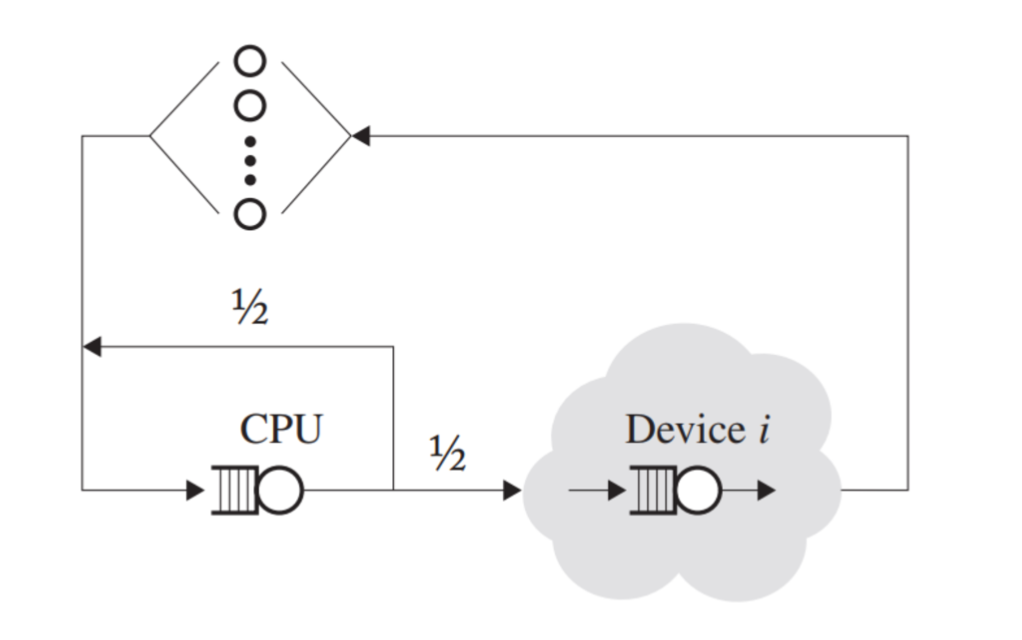
\includegraphics[width=0.7\textwidth]{Content/figure-6.png}
	\end{center}
%	{
%		\small
%		\bibliographystyle{ieeetr-fa}
%		\bibliography{MyReferences}
%	}
\end{document}